%%%%%%%%%%%%%%%%%%%%%%%%%%%%%%%%%%%%%%%%%%%%%%%%%%%%%%%%%%%%%%%%%%%%%%%%%%%%%%%
% PREAMBOLO COMUNE PER APPUNTI (Stile Scuro)
%
% Questo file contiene tutte le impostazioni e i pacchetti comuni.
% NON contiene \begin{document} o \end{document}.
%
% Istruzioni per la compilazione del file principale:
% pdflatex -shell-escape nomefile_principale.tex
%%%%%%%%%%%%%%%%%%%%%%%%%%%%%%%%%%%%%%%%%%%%%%%%%%%%%%%%%%%%%%%%%%%%%%%%%%%%%%%

\documentclass{article}

% --- Encoding e lingua ---
\usepackage[utf8]{inputenc}
\usepackage[italian]{babel}

% --- Margini e layout ---
\usepackage{geometry}
\geometry{a4paper, margin=1in}

% --- Font sans-serif (come Helvetica) ---
\usepackage[scaled]{helvet}
\renewcommand{\familydefault}{\sfdefault}
\usepackage[T1]{fontenc}

% --- Matematica ---
\usepackage{amsmath}
\usepackage{amssymb}

% --- Liste personalizzate ---
\usepackage{enumitem}
% \setlist{nosep}

% --- Immagini e Grafica ---
\usepackage{float}
% \usepackage{graphicx}
\usepackage{tikz}
\usetikzlibrary{shapes.geometric, positioning, arrows.meta, calc, fit, backgrounds, patterns, decorations.pathreplacing}

% --- Tabelle Avanzate ---
\usepackage{array}
\usepackage{booktabs}
\usepackage{longtable}

% --- Hyperlink e Metadati PDF ---
\usepackage{hyperref}

\hypersetup{
    colorlinks=true,
    linkcolor=white,
    filecolor=magenta,
    urlcolor=cyan,
    citecolor=green,
    % pdftitle, pdfauthor, ecc. verranno impostati nel file principale
    pdfpagemode=FullScreen,
    bookmarksopen=true,
    bookmarksnumbered=true
}

% --- Licenza del documento ---
\usepackage[
  type={CC},
  modifier={by-sa},
  version={4.0},
]{doclicense}

% --- Colori e Sfondo Nero ---
\usepackage{xcolor}
\pagecolor{black}
\color{white}

% --- Evidenziazione del Codice ---
\usepackage{minted}
\setminted{
    frame=lines,
    framesep=2mm,
    fontsize=\small,
    breaklines=true,
    style=monokai,
    bgcolor=black!80
}
\usemintedstyle{monokai}

% --- Comandi personalizzati per algebra relazionale ---
\newcommand{\Rel}[1]{\textit{#1}} % Per i nomi delle relazioni
\newcommand{\Attr}[1]{\textsf{#1}} % Per i nomi degli attributi

\newcommand{\myunion}{\cup}
\newcommand{\myintersection}{\cap}
\newcommand{\mydifference}{-}
\newcommand{\myrename}[2]{\rho_{#1}(#2)}
\newcommand{\myselectop}[2]{\sigma_{#1}(#2)}
\newcommand{\myproject}[2]{\pi_{#1}(#2)}
\newcommand{\mycartesian}{\times}
\newcommand{\mynaturaljoin}{\bowtie} % Usare \Join da amssymb se disponibile e preferito
\newcommand{\mythetajoin}[3]{#1 \bowtie_{#2} #3} % R1 \bowtie_cond R2

% --- Comandi personalizzati per logica ---
\newcommand{\mylandop}{\wedge}
\newcommand{\myvel}{\vee}
\newcommand{\mynegop}{\neg}
\newcommand{\myforallop}{\forall}
\newcommand{\myexistsop}{\exists}

% --- Join esterni (outer join) ---
% Definizione standard per i join esterni
\def\ojoin{\setbox0=\hbox{$\mynaturaljoin$}%
	\rule[-.02ex]{.25em}{.4pt}\llap{\rule[\ht0]{.25em}{.4pt}}}
\newcommand{\myleftouterjoin}{\mathbin{\ojoin\mkern-5.8mu\mynaturaljoin}}
\newcommand{\myrightouterjoin}{\mathbin{\mynaturaljoin\mkern-5.8mu\ojoin}}
\newcommand{\myfullouterjoin}{\mathbin{\ojoin\mkern-5.8mu\mynaturaljoin\mkern-5.8mu\ojoin}}



% --- Titolo ---
\title{Protocolli MAC Wireless}
\author{Basato sulle slide del Prof. Luciano Bononi}
\date{\today}

\begin{document}

\maketitle
\tableofcontents
\newpage

\section{Introduzione al Livello MAC Wireless}
Il livello MAC (Medium Access Control) nei sistemi wireless ha ruoli fondamentali per gestire l'accesso al mezzo trasmissivo condiviso (l'etere).

\subsection{Ruoli del Livello MAC Wireless}
\begin{itemize}
    \item \textbf{Controllo dell'Accesso al Canale Condiviso:}
    \begin{itemize}
        \item La trasmissione wireless è intrinsecamente \textit{broadcast}: tutti nel raggio d'azione possono ricevere.
        \item Questo porta a \textit{collisioni di segnale}: un problema sia temporale (chi trasmette quando) sia spaziale (chi trasmette dove).
        \item \textbf{Obiettivo principale}: Decidere chi trasmette, quando e (in alcuni contesti avanzati) dove.
        \item \textbf{Assenza di Collision Detection (CD)}: A differenza delle reti cablate (Ethernet), nelle reti wireless è difficile per un trasmettitore rilevare una collisione mentre sta trasmettendo. Il segnale emesso è molto più forte di qualsiasi segnale ricevuto, mascherando la collisione. Quindi, si punta sull'evitare le collisioni (\textit{Collision Avoidance - CA}).
    \end{itemize}
    \item \textbf{Utilizzo delle Scarse Risorse:}
    \begin{itemize}
        \item \textit{Capacità del canale (Channel capacity)} e \textit{consumo energetico (battery power)} sono limitati e preziosi. Il MAC deve ottimizzarne l'uso.
    \end{itemize}
    \item \textbf{Performance e QoS (Quality of Service):}
    \begin{itemize}
        \item Il MAC influenza le prestazioni percepite sia a livello di sistema (efficienza generale) sia a livello utente (es. ritardo, throughput per una specifica applicazione).
    \end{itemize}
    \item \textbf{Organizzazione dei Frame e Gestione delle Informazioni:}
    \begin{itemize}
        \item Gestione delle informazioni sia all'interno del livello MAC (\textit{intra-layer}) sia tra livelli diversi (\textit{inter-layer}).
        \item \textit{Cross-layering}: Principi per cui un livello può usare informazioni da altri livelli per ottimizzare il comportamento (es. il MAC usa info dal routing). Comporta il rischio di "spaghetti design" (architetture complesse e difficili da mantenere).
    \end{itemize}
\end{itemize}

\subsection{Collisione dei Segnali Wireless}
\begin{itemize}
    \item \textbf{Effetto Distruttivo sul Ricevitore:} Una collisione rende il segnale incomprensibile al ricevitore, causando spreco di canale (tempo perso) e di energia (trasmissioni inutili).
    \item \textbf{Collision Detection Non Pratica:} Come detto, difficile da implementare.
    \item \textbf{Strategie:}
    \begin{itemize}
        \item \textit{Collision Avoidance/Resolution}: Tecniche per prevenire o risolvere le collisioni.
        \item \textit{Contention Control sul Trasmettitore}: Il trasmettitore adotta meccanismi per ridurre la probabilità di collisione.
    \end{itemize}
    \item \textbf{Effetto Cattura (Capture Effect):}
    \begin{itemize}
        \item Se due segnali arrivano contemporaneamente, ma uno è significativamente più forte dell'altro, il ricevitore potrebbe riuscire a decodificare il segnale più forte.
        \item Può essere sfruttato per migliorare il riuso del canale.
        \item \textit{Esempio Pratico:} Immagina due persone che ti parlano contemporaneamente. Se una ti urla nell'orecchio e l'altra sussurra da lontano, probabilmente capirai chi urla.
    \end{itemize}
    \item \textbf{Dominio di Collisione (Collision Domain):} L'insieme di nodi che condividono lo stesso canale e le cui trasmissioni possono interferire tra loro.
    \begin{itemize}
        \item \textit{Space splitting, transitive relation}: La divisione spaziale e le relazioni transitive definiscono l'estensione del dominio di collisione.
    \end{itemize}
\end{itemize}

\subsection{Diagramma delle Collisioni}
Il diagramma seguente illustra come due domini di trasmissione possono sovrapporsi, creando una zona di potenziale collisione. I segnali diretti ai rispettivi ricevitori (indicati con un punto esclamativo) possono collidere se trasmessi contemporaneamente nello stesso spazio.

\begin{figure}[H]
\centering
\begin{tikzpicture}[scale=0.8, every node/.style={text=white}]
    % Primo trasmettitore e suo raggio
    \node (t1) at (-1.5,0) {\textbf{Tx1}};
    \node[nodo_testo, color=red, font=\Huge] at (-0.5,0.3) {\textbf{!}};
    \draw[red, thick] (t1) circle (1.5cm);
    \draw[linea, red, thick] (-1.5,0) -- (0,0) node[midway, above, nodo_testo, color=red] {Segnale 1};

    % Secondo trasmettitore e suo raggio
    \node (t2) at (1.5,0) {\textbf{Tx2}};
    \node[nodo_testo, color=blue, font=\Huge] at (0.5,0.3) {\textbf{!}};
    \draw[blue, thick] (t2) circle (1.5cm);
    \draw[linea, blue, thick] (1.5,0) -- (0,0) node[midway, above, nodo_testo, color=blue] {Segnale 2};

    % Area di sovrapposizione
    \begin{scope}
        \clip (t1) circle (1.5cm);
        \fill[yellow, opacity=0.3] (t2) circle (1.5cm);
    \end{scope}
    \node[nodo_testo] at (0,-2) {Area di potenziale collisione};
\end{tikzpicture}
\caption{Illustrazione di domini di collisione sovrapposti.}
\label{fig:collision_domain}
\end{figure}

\section{Classificazione dei Protocolli MAC Wireless}
I protocolli MAC possono essere classificati in base a come gestiscono l'accesso:

\begin{itemize}
    \item \textbf{Protocolli Basati su Contesa (Distributed Contention Based):} I nodi "competono" per accedere al canale.
    \begin{itemize}
        \item \textit{Deterministici:} L'accesso è determinato da un mapping di ID o un ordine fisso.
        \begin{itemize}
            \item Senza Coordinatore Centralizzato, allocazione statica delle risorse.
        \end{itemize}
        \item \textit{Probabilistici:} L'accesso è casuale, con meccanismi per risolvere le contese e le collisioni (es. ALOHA, CSMA).
        \begin{itemize}
            \item Senza Coordinatore Centralizzato, allocazione dinamica delle risorse.
            \item \textit{Esempio Pratico:} Pensa a una stanza affollata dove tutti vogliono parlare. Ognuno prova a parlare, e se due parlano insieme, si fermano, aspettano un tempo casuale e riprovano.
        \end{itemize}
    \end{itemize}
    \item \textbf{Protocolli Senza Contesa (Contention Free):} L'accesso al canale è regolato per evitare collisioni.
    \begin{itemize}
        \item \textit{Dinamici Distribuiti:}
        \begin{itemize}
            \item \textit{Implicit Reservation}: L'uso riuscito del canale può implicare una prenotazione per usi futuri.
            \item \textit{Token Based}: Un "gettone" logico circola tra i nodi; solo chi ha il gettone può trasmettere.
            \item Senza Coordinatore Centralizzato, allocazione dinamica delle risorse.
        \end{itemize}
        \item \textit{Statici Centralizzati:}
        \begin{itemize}
            \item \textit{Reservation Based}: Un coordinatore centrale assegna slot di tempo/frequenza/codice.
            \item Esempi: TDMA (Time Division Multiple Access), FDMA (Frequency DMA), CDMA (Code DMA).
            \item Con Coordinatore Centralizzato, allocazione statica (o semi-statica) delle risorse.
            \item \textit{Esempio Pratico (TDMA):} Un insegnante (coordinatore) dà a ogni studente (nodo) un preciso intervallo di tempo in cui può fare una domanda.
        \end{itemize}
    \end{itemize}
    \item \textbf{Cluster-based MAC}: Protocolli ibridi che possono formare gruppi (cluster) con un coordinatore locale.
\end{itemize}

\section{Prospettiva Evolutiva del MAC Distribuito (Dominio del Tempo)}
Si affronta il problema della \textit{vulnerabilità del frame} (rischio di collisione) e della necessità di una risoluzione distribuita.

\subsection{ALOHA}
Un nodo trasmette non appena ha dati. Se non riceve ACK, assume collisione e ritrasmette dopo backoff casuale.
\begin{itemize}
    \item \textbf{Tempo di vulnerabilità del frame = $2 \times \text{Tempo\_trasmissione\_frame}$.}
\end{itemize}

\begin{figure}[H]
\centering
\begin{tikzpicture}[nodo_base, font=\footnotesize, scale=0.8, transform shape]
    \node (ready) [nodo_base, diamond, aspect=2, fill=green!50!black] {Packet ready?};
    \node (transmit) [nodo_base, below=0.5cm of ready, fill=blue!50!black] {transmit};
    \node (wait_ack) [nodo_base, below=0.5cm of transmit] {wait for round-trip time};
    \node (ack_ok) [nodo_base, diamond, aspect=2, below=0.5cm of wait_ack, fill=green!50!black] {positive ack?};
    \node (delay_k) [nodo_base, right=2cm of transmit, fill=orange!50!black] {delay packet transmission k times};
    \node (backoff) [nodo_base, below=0.5cm of delay_k] {compute random backoff integer k};
    \node (end_yes) [nodo_base, left=2cm of ack_ok, opacity=0] {}; % Dummy for arrow

    \draw[linea] (ready) -- node[right, nodo_testo] {yes} (transmit);
    \draw[linea] (ready.east) -| node[above, nodo_testo] {no} ++(2.5,0) |- (ready.north);
    \draw[linea] (transmit) -- (wait_ack);
    \draw[linea] (wait_ack) -- (ack_ok);
    \draw[linea] (ack_ok.west) -| node[above, nodo_testo] {yes} (end_yes.east) -| (ready.west);
    \draw[linea] (ack_ok.east) -| node[above, nodo_testo] {no} (backoff.west);
    \draw[linea] (backoff) -- (delay_k);
    \draw[linea] (delay_k.north) |- (ready.north east);
\end{tikzpicture}
\caption{Diagramma di flusso del protocollo ALOHA.}
\label{fig:aloha_flow}
\end{figure}

\begin{figure}[H]
\centering
\begin{tikzpicture}[scale=0.9, every node/.style={text=white, font=\scriptsize}]
    % Asse tempo
    \draw[linea] (0,2.5) -- (7,2.5) node[right] {time};
    \node at (-0.5,2) {STA i};
    \draw[linea_doppia, red] (1,2.7) -- (3,2.7) node[midway, above] {Frame size};
    \node[blocco_tempo_verde, minimum width=2cm] at (1,1.8) {frame1};
    \node[blocco_tempo_verde, minimum width=1cm] at (5.5,1.8) {ok1};

    \draw[linea] (0,1.3) -- (7,1.3) node[right] {time};
    \node at (-0.5,0.8) {STA j};
    \node[blocco_tempo, minimum width=1cm] at (0.5,0.6) {early1};
    \node[blocco_tempo, minimum width=1.5cm] at (2.5,0.6) {late2};
    \node[blocco_tempo_hatch, minimum width=1.5cm] at (4,0.6) {pkt2 (coll)}; % Assuming collision

    \draw[linea] (0,0.1) -- (7,0.1) node[right] {time};
    \node at (-1, -0.4) {Collision domain};
    \node[blocco_tempo, minimum width=1cm] at (0.5,-0.6) {early1};
    \node[blocco_tempo_verde, minimum width=2cm] at (1.5,-0.6) {Frame1};
    \node[blocco_tempo, minimum width=1.5cm] at (3.5,-0.6) {late2};
    \fill[red, opacity=0.3] (1.5,-0.6) rectangle (3.5,0); % Collision area
    \node[color=red] at (2.5, -0.9) {collision};
    \node[blocco_tempo_verde, minimum width=1cm] at (5.5,-0.6) {ok1};


    \draw[decorate, decoration={brace, amplitude=5pt}] (0.5,-1.2) -- (3.5,-1.2) node[midway, below=2pt] {Frame vulnerability time: twice the frame size};
    \draw[decorate,decoration={brace,amplitude=3pt}] (0.5,-0.7) -- (1.5,-0.7) node[midway,above=1pt,xshift=-5mm] {New1+frame1 coll.};
    \draw[decorate,decoration={brace,amplitude=3pt}] (1.5,-0.7) -- (3.5,-0.7) node[midway,above=1pt,xshift=5mm] {Frame1+New2 coll.};

\end{tikzpicture}
\caption{Vulnerabilità del frame in ALOHA.}
\label{fig:aloha_vuln}
\end{figure}


\subsection{Slotted ALOHA}
Il tempo è diviso in slot; trasmissione solo all'inizio di uno slot.
\begin{itemize}
    \item \textbf{Tempo di vulnerabilità del frame = $1 \times \text{Tempo\_trasmissione\_frame}$.}
\end{itemize}
Il diagramma di flusso è simile ad ALOHA, con l'aggiunta di "Wait for start of next slot" prima di trasmettere.

\begin{figure}[H]
\centering
\begin{tikzpicture}[scale=0.9, every node/.style={text=white, font=\scriptsize}]
    % Asse tempo con slot
    \foreach \x in {1,2,...,6} {
        \draw[gray!50] (\x,2.8) -- (\x, -1);
    }
    \draw[linea] (0,2.5) -- (7,2.5) node[right] {time};
    \node at (-0.5,2) {STA i};
    \draw[<->, red] (1,2.7) -- (2,2.7) node[midway, above] {Framesize};
    \draw[<->, orange] (2,2.8) -- (2.5,2.8) node[midway, above, yshift=2pt] {Prop. delay};
    \node[blocco_tempo_verde, minimum width=1cm] at (1,1.8) {frame1};
    \node[blocco_tempo_verde, minimum width=1cm] at (2.5,1.8) {frame1 (tx)}; % Assuming retransmit or next

    \draw[linea] (0,1.3) -- (7,1.3) node[right] {time};
    \node at (-0.5,0.8) {STA j};
    \draw[<->, blue] (1,1.5) -- (2,1.5) node[midway, above] {time slot};
    \node[blocco_tempo, minimum width=1cm] at (1,0.6) {frame2};
    \node[blocco_tempo_hatch, minimum width=1cm] at (3.5,0.6) {frame2 (tx)};


    \draw[linea] (0,0.1) -- (7,0.1) node[right] {time};
    \node at (-1, -0.4) {Collision domain};
    \node[blocco_tempo_verde, minimum width=1cm] at (1,-0.6) {frame1};
    \fill[red, opacity=0.3] (1,-0.6) rectangle (2,0); % Collision frame2 started in same slot
    \node[color=red] at (1.5, -0.9) {collision};
    \node[blocco_tempo_verde, minimum width=1cm] at (2.5,-0.6) {frame1 (ok)}; % this frame1 is ok
    \node[blocco_tempo_hatch, minimum width=1cm] at (3.5,-0.6) {frame2 (ok)};

    \draw[decorate, decoration={brace, amplitude=5pt}] (1,-1.2) -- (2,-1.2) node[midway, below=2pt] {Frame1+frame2 collision};
    \node at (3.5, -1.5) {Vulnerability time: frame size (slot + propagation)};
\end{tikzpicture}
\caption{Vulnerabilità del frame in Slotted ALOHA.}
\label{fig:slotted_aloha_vuln}
\end{figure}

\subsection{CSMA (Carrier Sense Multiple Access)}
Un nodo ascolta ("carrier sense") il canale prima di trasmettere.
\begin{itemize}
    \item \textbf{Problema:} Ritardo di propagazione.
    \item \textbf{Tempo di vulnerabilità del frame = $2 \times \text{Ritardo\_propagazione}$.}
\end{itemize}
Il diagramma di flusso aggiunge un controllo "Channel Busy?" prima di trasmettere.

\begin{figure}[H]
\centering
\begin{tikzpicture}[scale=0.9, every node/.style={text=white, font=\scriptsize}]
    % Asse tempo
    \draw[linea] (0,2.5) -- (7,2.5) node[right] {time};
    \node at (-0.5,2) {STA i};
    \draw[<->, red] (1,2.7) -- (3,2.7) node[midway, above] {Frame size};
    \node[blocco_tempo_verde, minimum width=2cm] at (1,1.8) {frame1};
    \node[blocco_tempo_verde, pattern=north east lines, pattern color=gray, minimum width=2cm] at (3.5,1.8) {frame1 (tx)};

    \draw[linea] (0,1.3) -- (7,1.3) node[right] {time};
    \node at (-0.5,0.8) {STA j};
    \draw[<->, orange] (0.5,1.5) -- (1.5,1.5) node[midway, above] {Prop. delay};
    \node[blocco_tempo, minimum width=1cm] at (0.5,0.6) {early2};
    \node[blocco_tempo, minimum width=1cm] at (1.5,0.6) {late2}; % This one collides
    \node at (3,1.0) {Frame1 detected}; \draw[->, dashed, thick, red] (3,0.9) -- (1.5,1.9); % Point to frame1 start
    \node[blocco_tempo_hatch, minimum width=1cm] at (4.5,0.6) {late2 (coll)};

    \draw[linea] (0,0.1) -- (7,0.1) node[right] {time};
    \node at (-1, -0.4) {Collision domain};
    \node[blocco_tempo, minimum width=1cm] at (0.5,-0.6) {early2};
    \node[blocco_tempo_verde, minimum width=0.5cm, fill=red!70!black] at (1.5,-0.6) {}; % Part of frame1
    \node[blocco_tempo, minimum width=1cm, fill=red!70!black, xshift=0.5cm] at (1.5,-0.6) {}; % late2 over part of frame1
    \node[blocco_tempo_verde, minimum width=1.5cm, xshift=1cm] at (1.5,-0.6) {}; % Rest of frame1
    \node[color=red] at (2,-0.9) {collision};
    \node[blocco_tempo_verde, pattern=north east lines, pattern color=gray, minimum width=2cm] at (3.5,-0.6) {frame1 (ok)};

    \draw[decorate,decoration={brace,amplitude=3pt,mirror}] (0.5,-1.2) -- (1.5,-1.2) node[midway,below=1pt] {Frame1+early2 vuln.};
    \draw[decorate,decoration={brace,amplitude=3pt,mirror}] (1.5,-1.2) -- (2.5,-1.2) node[midway,below=1pt] {Frame1+late2 vuln.};
    \node at (3.5, -1.6) {Frame vulnerability time: twice the propagation delay};
\end{tikzpicture}
\caption{Vulnerabilità del frame in CSMA.}
\label{fig:csma_vuln}
\end{figure}

\subsection{Slotted CSMA}
Combina CSMA con slot temporali.
\begin{itemize}
    \item \textbf{Tempo di vulnerabilità del frame = $1 \times \text{Ritardo\_propagazione}$.}
\end{itemize}

\subsection{CSMA/CD (Collision Detection)}
Ascolta prima e durante la trasmissione. Non pratico in wireless.

\subsection{CSMA/CA (Collision Avoidance)}
Tecnica principale nelle reti wireless. Include risoluzione e controllo delle contese.

\subsection{Comparazione del Throughput}
Un grafico tipico (Figura \ref{fig:throughput_comparison}) mostra che, in termini di throughput massimo:
Slotted CSMA > Pure CSMA > Slotted ALOHA > Pure ALOHA.
Tutti questi protocolli soffrono di un calo di throughput ad alto carico.

\begin{figure}[H]
\centering
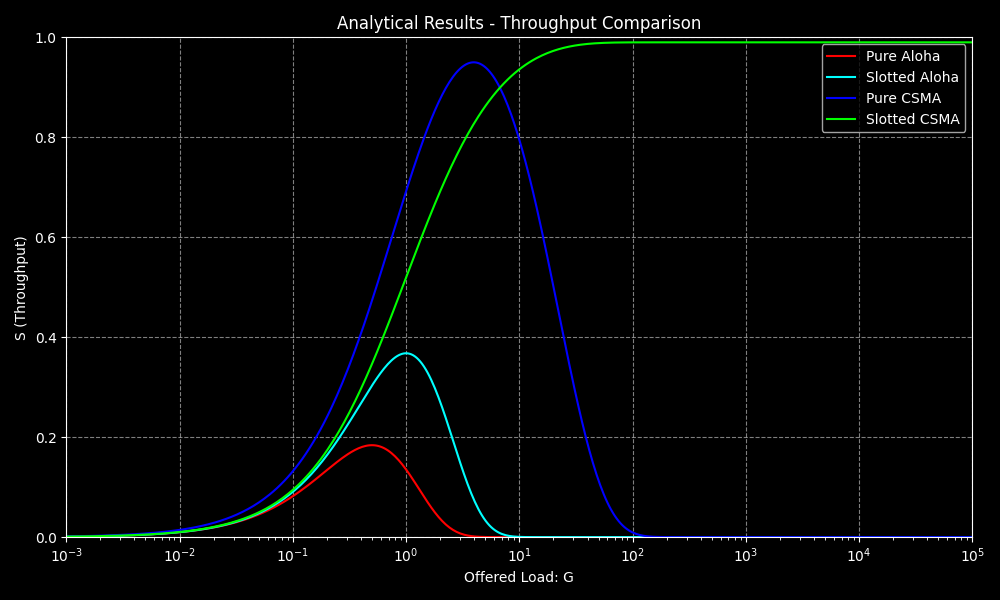
\includegraphics[width=0.8\textwidth]{images/throughput_comparison.png}
\caption{Comparazione teorica del throughput per diversi protocolli MAC.}
\label{fig:throughput_comparison}
\end{figure}


\section{Prospettiva Evolutiva del MAC Distribuito (Dominio dello Spazio)}
Affronta problemi come il terminale nascosto e esposto. Soluzione principale: RTS/CTS.

\subsection{Problema del Terminale Nascosto e Esposto}
\begin{itemize}
    \item \textbf{Terminale Nascosto:} A e C non si sentono, ma entrambi vogliono trasmettere a B. Collisione su B.
    \begin{itemize}
        \item \textbf{Soluzione con RTS/CTS:} A invia RTS a B. B risponde con CTS. C sente CTS e si astiene.
    \end{itemize}
    \item \textbf{Terminale Esposto:} B trasmette ad A. C (nel raggio di B) vuole trasmettere a D (fuori dal raggio di B). C sente B e non trasmette, sprecando un'opportunità.
\end{itemize}

\begin{figure}[H]
\centering
\begin{tikzpicture}[scale=0.7, every node/.style={text=white, font=\scriptsize}]
    % Scenario Sinistra: Collision on C (Hidden Terminal Problem)
    \node at (-3, 2.5) {Collision on C (Hidden Terminal)};
    \node (A1) [circle, draw, minimum size=0.5cm] at (-4,1) {A};
    \node (C1) [circle, draw, minimum size=0.5cm] at (-2,1) {C};
    \node (B1) [circle, draw, minimum size=0.5cm] at (-3,0) {B};
    \node (D1) [circle, draw, minimum size=0.5cm] at (-1,0) {D};

    \draw[linea, thick, red] (A1) -- (C1) node[midway, above] {A to C};
    \draw[linea, dotted, thick, blue] (B1) -- (C1) node[midway, left] {B to C (collides)};
    \draw[dashed, gray] (A1) ellipse (1.5cm and 1cm); % Range A
    \draw[dashed, gray] (B1) ellipse (1.5cm and 1cm); % Range B

    % Scenario Destra: RTS/CTS Solution
    \node at (3, 2.5) {Solution with RTS/CTS};
    \node (A2) [circle, draw, minimum size=0.5cm] at (1,0.5) {A};
    \node (C2) [circle, draw, minimum size=0.5cm] at (3,1) {C}; % Receiver
    \node (B2) [circle, draw, minimum size=0.5cm] at (5,0.5) {B}; % Hidden from A, hears CTS

    \draw[dashed, pink, fill=pink!30!black, opacity=0.7] (A2) circle (1.5cm); % A's range
    \draw[dashed, green, fill=green!30!black, opacity=0.7] (C2) circle (1.5cm); % C's range (receiver)
    \draw[dashed, orange, fill=orange!30!black, opacity=0.7] (B2) circle (1.5cm); % B's range

    \node at (A2) [above right=0.1cm of A2] {A};
    \node at (C2) [above right=0.1cm of C2] {C};
    \node at (B2) [above right=0.1cm of B2] {B};

    \draw[linea, thick, red] (A2) -- (C2) node[midway, above, sloped] {RTS};
    \draw[linea, thick, blue] (C2) -- (A2) node[midway, below, sloped] {CTS};
    \draw[linea, thick, blue, dashed] (C2) -- (B2) node[midway, below, sloped] {CTS}; % B hears CTS

    % Timeline sotto
    \draw[linea] (1,-1.5) -- (6,-1.5) node[right] {Time};
    \draw[linea] (0.5,-1) -- (0.5,-3) node[below] {Space};
    \node[blocco_tempo_rosso, minimum width=0.5cm, minimum height=0.2cm] at (1.5, -1.8) {RTS};
    \node[blocco_tempo, minimum width=0.5cm, minimum height=0.2cm] at (2.2, -2.1) {CTS};
    \node[blocco_tempo_verde, minimum width=1.5cm, minimum height=0.2cm] at (3, -1.8) {Data};
    \node[nodo_testo, anchor=east] at (1.4, -1.8) {A:};
    \node[nodo_testo, anchor=east] at (1.4, -2.1) {C:};
    \node[nodo_testo, anchor=east] at (1.4, -2.4) {B: (defers)};
    \draw[gray, dashed] (2.2,-2.4) -- (4.5,-2.4); % B defers
\end{tikzpicture}
\caption{Terminale Nascosto e soluzione RTS/CTS.}
\label{fig:hidden_terminal_rts_cts}
\end{figure}

\subsection{RTS/CTS - Svantaggi}
\begin{itemize}
    \item Non è una soluzione garantita (collisioni di RTS).
    \item Overhead aggiuntivo.
    \item Asimmetria di potenza e range (raggio di interferenza > raggio di trasmissione).
\end{itemize}
\begin{figure}[H]
\centering
\begin{tikzpicture}[scale=0.7, every node/.style={text=white}]
    \node (A) [circle, draw, fill=pink!50!black, minimum size=1cm, label=A] at (0,1.5) {};
    \node (C) [circle, draw, fill=green!50!black, minimum size=1cm, label=C] at (2,1.5) {};
    \node (B) [circle, draw, fill=blue!50!black, minimum size=1cm, label=B] at (4,1.5) {};
    \node (D) [circle, draw, fill=teal!50!black, minimum size=3cm, label=below:D] at (2,0) {};

    \draw[linea, thick] (A) -- (C) node[midway, above] {RTS};
    \draw[linea, thick] (C) -- (A) node[midway, below] {CTS};
    \draw[linea, thick, dashed] (C) -- (B) node[midway, above] {CTS};
    \node[nodo_testo, align=center] at (2,-2) {D potrebbe essere interferito o \\ interferire inutilmente se l'asimmetria di potenza \\ o il range di interferenza sono significativi.};
\end{tikzpicture}
\caption{Potenziali svantaggi di RTS/CTS con un nodo D.}
\label{fig:rts_cts_drawbacks}
\end{figure}

\subsection{Evoluzione dei Protocolli basati su RTS/CTS}
\begin{itemize}
    \item \textbf{MACA (Multiple Access with Collision Avoidance):} RTS/CTS, no carrier sense. Contesa sul ricevitore.
    \item \textbf{MACAW (MACA for Wireless):} No carrier sense, introduce ACK esplicito (RTS-CTS-DATA-ACK). Backoff MILD/BEB.
    \item \textbf{FAMA (Floor Acquisition Multiple Access):} Reintroduce carrier sense prima di RTS/CTS. Concetto di "floor acquisition".
\end{itemize}
I diagrammi per MACA, MACAW e FAMA (slide 18-20) sono simili a Figura \ref{fig:hidden_terminal_rts_cts} (scenario a destra), con l'aggiunta/rimozione del carrier sense e dell'ACK.

\section{Problemi Tempo/Spazio in Reti Ad Hoc Multi-hop}
In catene multi-hop (A->B->C), sorgono problemi di auto-contesa:
\begin{itemize}
    \item \textbf{Auto-contesa Inter-stream:} Dati (A->B) vs ACK (B->A) attorno a B.
    \item \textbf{Auto-contesa Intra-stream:} B riceve da A e trasmette a C; la sua trasmissione può interferire con la ricezione.
    \item \textbf{Coordinazione:} Soluzioni proposte includono fast forward, quick exchange, flow numbering.
\end{itemize}

\section{CSMA/CA: Lo Standard IEEE 802.11 (Wireless LAN)}
Un protocollo MAC con due funzioni di coordinamento in una struttura di superframe:
\begin{itemize}
    \item \textbf{DCF (Distributed Coordination Function):} Base, obbligatoria. Reti Ad-Hoc e contesa. Controllo distribuito, CSMA/CA con BEB.
    \item \textbf{PCF (Point Coordination Function):} Opzionale. Richiede Point Coordinator (AP). Controllo centralizzato, polling, QoS "soft".
\end{itemize}

\subsection{Architettura del Protocollo MAC IEEE 802.11}
\begin{figure}[H]
\centering
\begin{tikzpicture}[nodo_base, scale=0.9, transform shape, font=\scriptsize]
    \node (phy) [minimum width=8cm, minimum height=1cm, fill=orange!60!black] {Physical Layer (PHY)};
    \node (dcf) [above=0cm of phy.west, anchor=south west, minimum width=8cm, minimum height=1cm, fill=cyan!60!black] {Distributed Coordination Function (DCF)};
    \node (pcf) [above=0cm of dcf.north west, anchor=south west, minimum width=4cm, minimum height=1cm, fill=green!60!black] {Point Coordination Function (PCF)};

    \node (mac_sub) [left=0.5cm of dcf.west, anchor=east, rotate=90] {MAC sublayer};
    \draw[linea_doppia] ($(mac_sub.south)+(0,0.2)$) -- ($(mac_sub.north)-(0,0.2)$);

    \node (cont_free_serv) [ellipse, draw=white, fill=purple!60!black, minimum width=3.5cm, above left=0.2cm and 1cm of pcf.north east] {contention free services};
    \node (cont_based_serv) [ellipse, draw=white, fill=magenta!60!black, minimum width=3.5cm, above right=0.2cm and 1cm of dcf.north east] {Contention based services};

    \draw[linea, ultra thick, red!80!white] (cont_free_serv.south) -- (pcf.north);
    \draw[linea, ultra thick, red!80!white] (cont_based_serv.south) -- (dcf.north);
    % Simulare frecce multiple
    \foreach \i in {-0.3, -0.1, 0.1, 0.3} {
        \draw[linea, thick, yellow!80!white] ($(cont_free_serv.south)+(\i,0)$) -- ($(pcf.north)+(\i,0)$);
        \draw[linea, thick, yellow!80!white] ($(cont_based_serv.south east)+(\i-0.5,0)$) -- ($(dcf.north east)+(\i-0.5,0)$);
    }
    \node (fam) [right=1cm of dcf.east, anchor=west] {Fundamental Access Method};
    \draw[linea] (dcf.east) -- (fam.west);
\end{tikzpicture}
\caption{Architettura del protocollo MAC IEEE 802.11.}
\label{fig:mac_architecture}
\end{figure}

\subsection{Point Coordinated Mode (PCF)}
Servizio opzionale, senza contesa, gestito dall'AP (Point Coordinator) tramite Beacon e polling durante il CFP (Contention Free Period).
\begin{figure}[H]
\centering
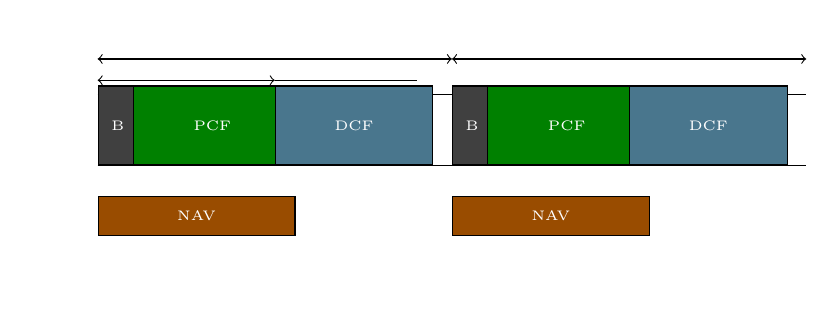
\begin{tikzpicture}[scale=0.9, every node/.style={text=white, font=\tiny}]
    % Superframe structure
    \draw (0,1) -- (10,1);
    \draw (0,0) -- (10,0);

    \node[rectangle, draw, fill=gray!50!black, minimum height=1cm, minimum width=0.5cm, anchor=south west] (b1) at (0,0) {B};
    \node[rectangle, draw, fill=green!50!black, minimum height=1cm, minimum width=2cm, anchor=south west] (pcf1) at (0.5,0) {PCF};
    \node[rectangle, draw, fill=cyan!50!black, minimum height=1cm, minimum width=2cm, anchor=south west] (dcf1) at (2.5,0) {DCF};

    \node[rectangle, draw, fill=gray!50!black, minimum height=1cm, minimum width=0.5cm, anchor=south west] (b2) at (5,0) {B};
    \node[rectangle, draw, fill=green!50!black, minimum height=1cm, minimum width=2cm, anchor=south west] (pcf2) at (5.5,0) {PCF};
    \node[rectangle, draw, fill=cyan!50!black, minimum height=1cm, minimum width=2cm, anchor=south west] (dcf2) at (7.5,0) {DCF};

    \draw[<->] (0,1.2) -- (2.5,1.2) node[midway, above] {CFP};
    \draw (2.5,1.2) -- (4.5,1.2) node[midway, above] {CP}; % CFP Repetition Interval
    \draw[<->] (0,1.5) -- (5,1.5) node[midway, above] {CFP Repetition Interval};
    \draw[<->] (5,1.5) -- (10,1.5) node[midway, above] {CFP Repetition Interval};


    % NAV
    \node[rectangle, draw, fill=orange!60!black, minimum height=0.5cm, minimum width=2.5cm, anchor=south west] (nav1) at (0,-1) {NAV};
    \node[rectangle, draw, fill=orange!60!black, minimum height=0.5cm, minimum width=2.5cm, anchor=south west] (nav2) at (5,-1) {NAV};
    \node at (2.5,-1.5) {NAV (Network Allocation Vector) indica canale occupato};
\end{tikzpicture}
\caption{Struttura del Superframe IEEE 802.11 con PCF e DCF, e NAV.}
\label{fig:superframe_nav}
\end{figure}

\subsection{Controllo DCF e PCF: Interframe Spaces (IFS)}
Priorità di accesso gestita da intervalli: SIFS < PIFS < DIFS.
\begin{figure}[H]
\centering
\begin{tikzpicture}[font=\tiny, scale=0.85, transform shape]
    % Timeline
    \draw[linea] (0,0) -- (14,0);

    % Scenario 1: DCF only
    \node[nodo_testo, above=0.8cm of {(-0.5,0)}] {DCF time (scenario 1: no PCF takes control)};
    \node[blocco_tempo_verde, minimum width=2cm] (dcf_t1) at (0,-0.3) {DCF Trans. 1};
    \node[blocco_tempo, minimum width=0.5cm] (sifs1) at ($(dcf_t1.south east)+(0.05,0)$) {SIFS};
    \node[blocco_tempo_rosso, minimum width=1cm] (ack1) at ($(sifs1.south east)+(0.05,0)$) {ack};
    \node[blocco_tempo, minimum width=1cm, fill=purple!60!black] (difs1) at ($(ack1.south east)+(0.05,0)$) {DIFS};
    \node[blocco_tempo_hatch, minimum width=1.5cm] (backoff1) at ($(difs1.south east)+(0.05,0)$) {Backoff};
    \node[blocco_tempo_verde, minimum width=2cm] (dcf_t2) at ($(backoff1.south east)+(0.05,0)$) {DCF Trans. 2};
    \node[blocco_tempo, minimum width=0.5cm] (sifs2) at ($(dcf_t2.south east)+(0.05,0)$) {SIFS};
    \node[blocco_tempo_rosso, minimum width=1cm] (ack2) at ($(sifs2.south east)+(0.05,0)$) {ack};
    \node[blocco_tempo, minimum width=1cm, fill=purple!60!black] (difs2) at ($(ack2.south east)+(0.05,0)$) {DIFS};
    \node[blocco_tempo_verde, minimum width=1cm, fill=yellow!60!black] at ($(difs2.south east)+(0.05,0)$) {DCF};

    % Scenario 2: PCF takes control
    \node[nodo_testo, above=0.8cm of {(0, -1.8)}] {PCF (polling based) time (scenario 2)};
    \node[blocco_tempo, fill=orange!60!black, minimum width=0.8cm] (poll_start) at (0,-2.1) {Poll}; % Start of PCF
    \node[blocco_tempo, minimum width=0.5cm] (sifs_pcf1) at ($(poll_start.south east)+(0.05,0)$) {SIFS};
    \node[blocco_tempo_verde, minimum width=1.5cm] (pcf_t1) at ($(sifs_pcf1.south east)+(0.05,0)$) {Poll trans. 1};
    \node[blocco_tempo, minimum width=0.5cm] (sifs_pcf2) at ($(pcf_t1.south east)+(0.05,0)$) {SIFS};
    \node[blocco_tempo_rosso, minimum width=1cm] (ack_pcf1) at ($(sifs_pcf2.south east)+(0.05,0)$) {ack};
    \node[blocco_tempo, minimum width=0.8cm, fill=gray!60!black] (pifs1) at ($(ack_pcf1.south east)+(0.05,0)$) {PIFS}; % AP waits PIFS
    \node[blocco_tempo_verde, minimum width=1.5cm] (pcf_t2) at ($(pifs1.south east)+(0.05,0)$) {Poll trans. 2};
    \node[blocco_tempo, minimum width=0.5cm] (sifs_pcf3) at ($(pcf_t2.south east)+(0.05,0)$) {SIFS};
    \node[blocco_tempo_rosso, minimum width=1cm] (ack_pcf2) at ($(sifs_pcf3.south east)+(0.05,0)$) {ack};
    \node[blocco_tempo, minimum width=1cm, fill=purple!60!black] (difs_after_pcf) at ($(ack_pcf2.south east)+(0.05,0)$) {DIFS};
    \node[nodo_testo, right=0.1cm of difs_after_pcf] {: restart DCF};
    \node[blocco_tempo_verde, minimum width=1cm, fill=yellow!60!black] at ($(difs_after_pcf.south east)+(0.55,0)$) {DCF};

    % Legenda
    \node[rectangle, fill=green!60!black, label={[text=white, font=\tiny]right:DCF/PCF Transmit}, minimum size=0.3cm] at (0,-3.5) {};
    \node[rectangle, fill=blue!70!black, label={[text=white, font=\tiny]right:SIFS}, minimum size=0.3cm] at (3,-3.5) {};
    \node[rectangle, fill=red!70!black, label={[text=white, font=\tiny]right:ACK/Poll}, minimum size=0.3cm] at (5,-3.5) {};
    \node[rectangle, fill=purple!60!black, label={[text=white, font=\tiny]right:DIFS}, minimum size=0.3cm] at (7.5,-3.5) {};
    \node[rectangle, fill=gray!60!black, label={[text=white, font=\tiny]right:PIFS}, minimum size=0.3cm] at (9.5,-3.5) {};
    \node[rectangle, pattern=north east lines, pattern color=gray, label={[text=white, font=\tiny]right:Backoff (contention)}, minimum size=0.3cm] at (11.5,-3.5) {};
\end{tikzpicture}
\caption{Controllo DCF e PCF tramite Interframe Spaces (IFS).}
\label{fig:ifs_control}
\end{figure}

\subsection{Distributed Coordination Function (DCF) in dettaglio}
Modalità CSMA/CA con Backoff Esponenziale Binario (BEB) su tempo idle slottato.
\begin{figure}[H]
\centering
\begin{tikzpicture}[font=\tiny, scale=0.9, transform shape]
    % Timeline
    \draw[linea] (0,0) -- (12,0);
    \node[blocco_tempo, minimum width=2cm, fill=orange!60!black] (busy) at (0,-0.3) {Medium Busy};
    \node[blocco_tempo, minimum width=1cm, fill=purple!60!black] (difs) at ($(busy.south east)+(0.1,0)$) {DIFS};

    % Backoff slots
    \node (backoff_start) at ($(difs.east)+(0.1,0.15)$) {};
    \foreach \i [count=\xi from 1] in {1,...,4} {
        \node (s\xi) [blocco_tempo, minimum width=0.5cm, fill=gray!60!black, minimum height=0.2cm, anchor=west] at ($(backoff_start)+(\i*0.6-0.6,0)$) {Slot \xi};
        \draw[gray!70] (s\xi.south west) -- ++(0,-0.4);
        \ifnum\xi=4
             \node (backoff_end) at (s\xi.east) {};
        \fi
    }
    \draw[decorate, decoration={brace,amplitude=4pt,mirror}] (backoff_start) -- (backoff_end) node[midway, below=2pt] {Backoff period};
    \node[blocco_tempo_verde, minimum width=3cm] (pkt_tx) at ($(backoff_end)+(0.1,-0.3)$) {Packet Transmitted};
    \node[blocco_tempo, minimum width=0.5cm] (sifs_ack) at ($(pkt_tx.south east)+(0.1,0)$) {SIFS};
    \node[blocco_tempo_rosso, minimum width=1cm] (ack_rx) at ($(sifs_ack.south east)+(0.1,0)$) {ACK};
\end{tikzpicture}
\caption{Funzionamento base del DCF con backoff.}
\label{fig:dcf_basic}
\end{figure}

\subsection{Meccanismo di Accesso CSMA/CA (DCF)}
\begin{enumerate}
    \item \textbf{Medium Busy:} Se canale occupato, attendi che si liberi.
    \item \textbf{DIFS:} Attendi DIFS.
    \item \textbf{Back-off Window:} Scegli slot casuali da CW, decrementa contatore se canale libero, congela se occupato.
    \item \textbf{Packet Transmitted:} Trasmetti quando contatore è zero.
\end{enumerate}

\subsection{Procedura di Backoff DCF}
\begin{itemize}
    \item \textbf{Selezione Tempo di Backoff Casuale:} $\text{BackoffTime} = \text{random}(0, \text{CW}_i - 1) \times \text{SlotTime}$.
    $\text{CW}_i$ (Contention Window) raddoppia dopo ogni collisione ($\text{CW}_{\min} \le \text{CW}_i \le \text{CW}_{\max}$).
    \begin{center}
    \begin{tabular}{|c|c|c|c|c|c|c|c|}
        \hline
        \textbf{i} & 1 & 2 & 3 & 4 & 5 & 6 & 7 \\ \hline
        $\mathbf{CW_i}$ & 15 & 31 & 63 & 127 & 255 & 511 & 1023 \\ \hline
    \end{tabular}
    \end{center}
    (Valori $\text{CW}_{\min}$ tipici possono essere 15 o 31 a seconda dello standard fisico)
    \item \textbf{Riduzione Tempo di Backoff:} Dopo DIFS, decrementa per ogni slot idle.
    \item \textbf{Congelamento (Frozen):} Se mezzo occupato, sospendi backoff.
    \item \textbf{Trasmissione:} A backoff zero, trasmetti.
\end{itemize}

\subsection{DCF Basic Access: Panoramica}
\begin{itemize}
    \item \textbf{Trasmissione Riuscita:} Sorgente (DIFS, Backoff, DATA) -> Destinazione (SIFS, ACK).
    \item \textbf{Collisione (senza CD):} Pacchetti collidono. Lunghezza collisione = $\max(L_A, L_B, L_C, \dots)$. Mancanza di ACK segnala collisione.
\end{itemize}
\begin{figure}[H]
\centering
\begin{tikzpicture}[font=\tiny, scale=0.85, transform shape]
    % Success
    \node[nodo_testo, anchor=west] at (-1,1.5) {\textbf{Successful transmission:}};
    \draw[linea] (0,1) -- (7,1); \node[left] at (0,1) {Source};
    \node[blocco_tempo, fill=purple!60!black, minimum width=1cm] (d1) at (0.5,0.7) {DIFS};
    \node[blocco_tempo_verde, minimum width=2cm] (data) at ($(d1.south east)+(0.1,0)$) {DATA};
    \node[blocco_tempo, minimum width=0.5cm] (s1) at ($(data.south east)+(0.1,0)$) {SIFS};
    \node[blocco_tempo, fill=purple!60!black, minimum width=1cm] (d2) at ($(s1.south east)+(0.1,0)$) {DIFS};

    \draw[linea] (0,0) -- (7,0); \node[left] at (0,0) {Destination};
    \node[blocco_tempo_rosso, minimum width=1cm] (ack_s) at ($(s1.south)+(0,-0.3)$) {ACK}; % Aligned with SIFS end

    % Collision
    \node[nodo_testo, anchor=west] at (-1,-1) {\textbf{Collision: no CD}};
    \draw[linea] (0,-1.5) -- (7,-1.5); \node[left] at (0,-1.5) {Station A};
    \node[blocco_tempo, fill=purple!60!black, minimum width=0.8cm] (d_ca) at (0.5,-1.8) {DIFS};
    \node[blocco_tempo_verde, minimum width=2.5cm] (la) at ($(d_ca.south east)+(0.1,0)$) {$L_A$};

    \draw[linea] (0,-2.5) -- (7,-2.5); \node[left] at (0,-2.5) {Station B};
    \node[blocco_tempo, fill=purple!60!black, minimum width=0.8cm] (d_cb) at (0.5,-2.8) {DIFS};
    \node[blocco_tempo, minimum width=1.5cm, fill=blue!60!black] (lb) at ($(d_cb.south east)+(0.3,0)$) {$L_B$}; % Slightly offset

    \draw[linea] (0,-3.5) -- (7,-3.5); \node[left] at (0,-3.5) {Station C};
    \node[blocco_tempo, fill=purple!60!black, minimum width=0.8cm] (d_cc) at (0.5,-3.8) {DIFS};
    \node[blocco_tempo, minimum width=1cm, fill=orange!60!black] (lc) at ($(d_cc.south east)+(0.6,0)$) {$L_C$}; % Further offset

    % Collision length indication
    \coordinate (coll_start) at ($(d_ca.east)+(0.1,0.15)$);
    \coordinate (coll_end) at (la.east); % End of longest packet LA
    \draw[decorate, decoration={brace,amplitude=4pt}] (coll_start |- 0,-4.5) -- (coll_end |- 0,-4.5) node[midway, below=2pt] {COLLISION LENGTH = max($L_A,L_B,L_C$)};
    \node[nodo_testo, color=red, right=1cm of la] at (coll_end) {IEEE 802.11 no CD};
\end{tikzpicture}
\caption{DCF: Trasmissione riuscita e scenario di collisione.}
\label{fig:dcf_overview}
\end{figure}


\subsection{Controllo della Contesa in IEEE 802.11}
Alta contesa porta a molte collisioni e basso utilizzo del canale. Il BEB cerca di mitigare ciò.
Un grafico tipico (Figura \ref{fig:contention_control}) mostra che l'utilizzo del canale diminuisce all'aumentare del numero di stazioni.

\begin{figure}[H]
\centering
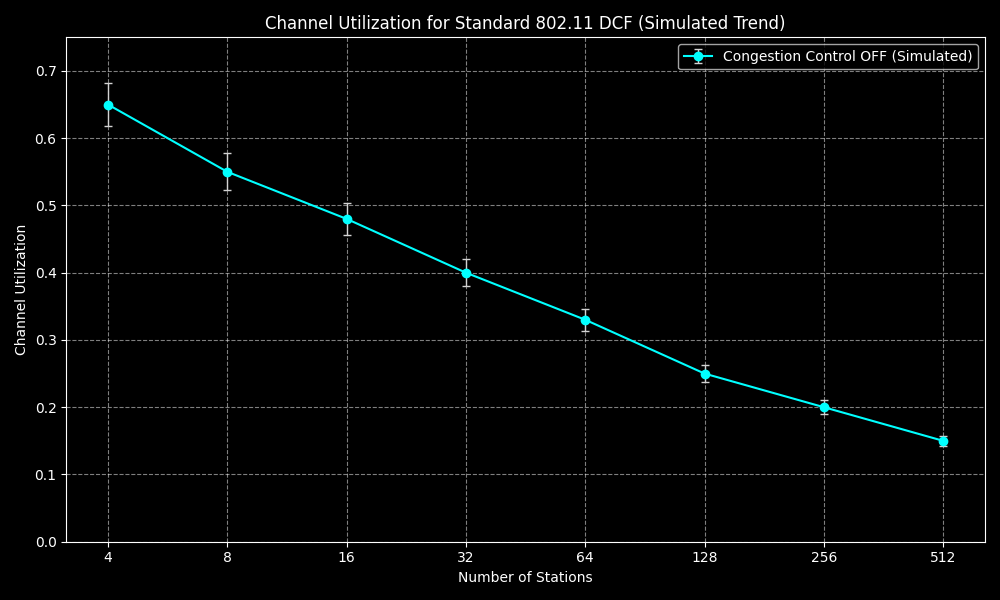
\includegraphics[width=0.8\textwidth]{images/contention_control.png}
\caption{Effetto della contesa sull'utilizzo del canale in IEEE 802.11 DCF.}
\label{fig:contention_control}
\end{figure}

\end{document}